% Created by tikzDevice version 0.12.6 on 2026-08-03 04:42:35
% !TEX encoding = UTF-8 Unicode
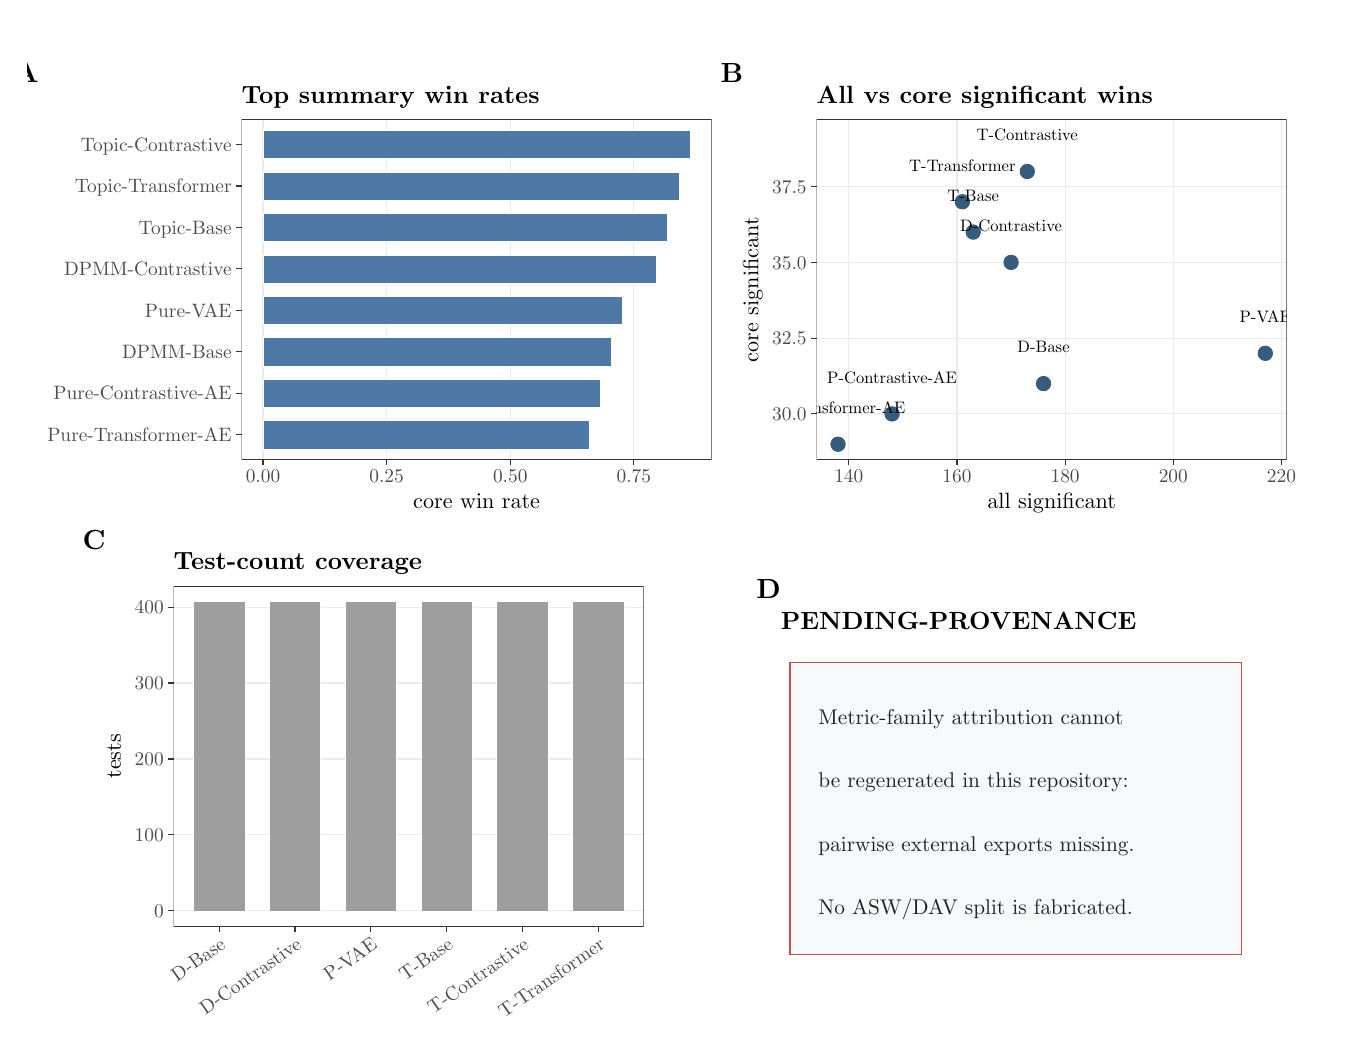
\begin{tikzpicture}[x=1pt,y=1pt]
\definecolor{fillColor}{RGB}{255,255,255}
\path[use as bounding box,fill=fillColor,fill opacity=0.00] (0,0) rectangle (473.86,364.00);
\begin{scope}
\path[clip] (  0.00,  0.00) rectangle (473.86,364.00);
\definecolor{drawColor}{RGB}{255,255,255}
\definecolor{fillColor}{RGB}{255,255,255}

\path[draw=drawColor,line width= 0.6pt,line join=round,line cap=round,fill=fillColor] (  0.00,  0.00) rectangle (473.86,364.00);
\end{scope}
\begin{scope}
\path[clip] (  5.50,182.00) rectangle (236.93,358.50);
\definecolor{drawColor}{RGB}{255,255,255}
\definecolor{fillColor}{RGB}{255,255,255}

\path[draw=drawColor,line width= 0.6pt,line join=round,line cap=round,fill=fillColor] (  5.50,182.00) rectangle (236.93,358.50);
\end{scope}
\begin{scope}
\path[clip] (236.93,182.00) rectangle (468.36,358.50);
\definecolor{drawColor}{RGB}{255,255,255}
\definecolor{fillColor}{RGB}{255,255,255}

\path[draw=drawColor,line width= 0.6pt,line join=round,line cap=round,fill=fillColor] (236.93,182.00) rectangle (468.36,358.50);
\end{scope}
\begin{scope}
\path[clip] (  0.00,186.43) rectangle (249.14,354.06);
\definecolor{drawColor}{RGB}{255,255,255}
\definecolor{fillColor}{RGB}{255,255,255}

\path[draw=drawColor,line width= 0.4pt,line join=round,line cap=round,fill=fillColor] ( -6.71,186.43) rectangle (249.14,354.06);
\end{scope}
\begin{scope}
\path[clip] ( 77.31,207.90) rectangle (247.14,330.76);
\definecolor{fillColor}{RGB}{255,255,255}

\path[fill=fillColor] ( 77.31,207.90) rectangle (247.14,330.76);
\definecolor{drawColor}{gray}{0.92}

\path[draw=drawColor,line width= 0.4pt,line join=round] ( 85.03,207.90) --
	( 85.03,330.76);

\path[draw=drawColor,line width= 0.4pt,line join=round] (129.70,207.90) --
	(129.70,330.76);

\path[draw=drawColor,line width= 0.4pt,line join=round] (174.38,207.90) --
	(174.38,330.76);

\path[draw=drawColor,line width= 0.4pt,line join=round] (219.05,207.90) --
	(219.05,330.76);
\definecolor{drawColor}{RGB}{255,255,255}
\definecolor{fillColor}{RGB}{78,121,167}

\path[draw=drawColor,line width= 0.2pt,fill=fillColor] ( 85.03,316.67) rectangle (239.42,326.86);

\path[draw=drawColor,line width= 0.2pt,fill=fillColor] ( 85.03,301.69) rectangle (235.31,311.88);

\path[draw=drawColor,line width= 0.2pt,fill=fillColor] ( 85.03,286.71) rectangle (231.20,296.90);

\path[draw=drawColor,line width= 0.2pt,fill=fillColor] ( 85.03,271.72) rectangle (227.09,281.91);

\path[draw=drawColor,line width= 0.2pt,fill=fillColor] ( 85.03,256.74) rectangle (214.94,266.93);

\path[draw=drawColor,line width= 0.2pt,fill=fillColor] ( 85.03,241.76) rectangle (211.01,251.95);

\path[draw=drawColor,line width= 0.2pt,fill=fillColor] ( 85.03,226.78) rectangle (206.90,236.96);

\path[draw=drawColor,line width= 0.2pt,fill=fillColor] ( 85.03,211.79) rectangle (202.79,221.98);
\definecolor{drawColor}{gray}{0.20}

\path[draw=drawColor,line width= 0.4pt,line join=round,line cap=round] ( 77.31,207.90) rectangle (247.14,330.76);
\end{scope}
\begin{scope}
\path[clip] (  0.00,  0.00) rectangle (473.86,364.00);
\definecolor{drawColor}{gray}{0.30}

\node[text=drawColor,anchor=base east,inner sep=0pt, outer sep=0pt, scale=  0.70] at ( 73.71,214.48) {Pure-Transformer-AE};

\node[text=drawColor,anchor=base east,inner sep=0pt, outer sep=0pt, scale=  0.70] at ( 73.71,229.46) {Pure-Contrastive-AE};

\node[text=drawColor,anchor=base east,inner sep=0pt, outer sep=0pt, scale=  0.70] at ( 73.71,244.44) {DPMM-Base};

\node[text=drawColor,anchor=base east,inner sep=0pt, outer sep=0pt, scale=  0.70] at ( 73.71,259.42) {Pure-VAE};

\node[text=drawColor,anchor=base east,inner sep=0pt, outer sep=0pt, scale=  0.70] at ( 73.71,274.41) {DPMM-Contrastive};

\node[text=drawColor,anchor=base east,inner sep=0pt, outer sep=0pt, scale=  0.70] at ( 73.71,289.39) {Topic-Base};

\node[text=drawColor,anchor=base east,inner sep=0pt, outer sep=0pt, scale=  0.70] at ( 73.71,304.37) {Topic-Transformer};

\node[text=drawColor,anchor=base east,inner sep=0pt, outer sep=0pt, scale=  0.70] at ( 73.71,319.36) {Topic-Contrastive};
\end{scope}
\begin{scope}
\path[clip] (  0.00,  0.00) rectangle (473.86,364.00);
\definecolor{drawColor}{gray}{0.20}

\path[draw=drawColor,line width= 0.4pt,line join=round] ( 75.31,216.89) --
	( 77.31,216.89);

\path[draw=drawColor,line width= 0.4pt,line join=round] ( 75.31,231.87) --
	( 77.31,231.87);

\path[draw=drawColor,line width= 0.4pt,line join=round] ( 75.31,246.85) --
	( 77.31,246.85);

\path[draw=drawColor,line width= 0.4pt,line join=round] ( 75.31,261.84) --
	( 77.31,261.84);

\path[draw=drawColor,line width= 0.4pt,line join=round] ( 75.31,276.82) --
	( 77.31,276.82);

\path[draw=drawColor,line width= 0.4pt,line join=round] ( 75.31,291.80) --
	( 77.31,291.80);

\path[draw=drawColor,line width= 0.4pt,line join=round] ( 75.31,306.78) --
	( 77.31,306.78);

\path[draw=drawColor,line width= 0.4pt,line join=round] ( 75.31,321.77) --
	( 77.31,321.77);
\end{scope}
\begin{scope}
\path[clip] (  0.00,  0.00) rectangle (473.86,364.00);
\definecolor{drawColor}{gray}{0.20}

\path[draw=drawColor,line width= 0.4pt,line join=round] ( 85.03,205.90) --
	( 85.03,207.90);

\path[draw=drawColor,line width= 0.4pt,line join=round] (129.70,205.90) --
	(129.70,207.90);

\path[draw=drawColor,line width= 0.4pt,line join=round] (174.38,205.90) --
	(174.38,207.90);

\path[draw=drawColor,line width= 0.4pt,line join=round] (219.05,205.90) --
	(219.05,207.90);
\end{scope}
\begin{scope}
\path[clip] (  0.00,  0.00) rectangle (473.86,364.00);
\definecolor{drawColor}{gray}{0.30}

\node[text=drawColor,anchor=base,inner sep=0pt, outer sep=0pt, scale=  0.70] at ( 85.03,199.48) {0.00};

\node[text=drawColor,anchor=base,inner sep=0pt, outer sep=0pt, scale=  0.70] at (129.70,199.48) {0.25};

\node[text=drawColor,anchor=base,inner sep=0pt, outer sep=0pt, scale=  0.70] at (174.38,199.48) {0.50};

\node[text=drawColor,anchor=base,inner sep=0pt, outer sep=0pt, scale=  0.70] at (219.05,199.48) {0.75};
\end{scope}
\begin{scope}
\path[clip] (  0.00,  0.00) rectangle (473.86,364.00);
\definecolor{drawColor}{RGB}{0,0,0}

\node[text=drawColor,anchor=base,inner sep=0pt, outer sep=0pt, scale=  0.80] at (162.23,190.20) {core win rate};
\end{scope}
\begin{scope}
\path[clip] (  0.00,  0.00) rectangle (473.86,364.00);
\definecolor{drawColor}{RGB}{0,0,0}

\node[text=drawColor,anchor=base west,inner sep=0pt, outer sep=0pt, scale=  0.90] at ( 77.31,336.74) {\bfseries Top summary win rates};
\end{scope}
\begin{scope}
\path[clip] (  0.00,  0.00) rectangle (473.86,364.00);
\definecolor{drawColor}{RGB}{0,0,0}

\node[text=drawColor,anchor=base,inner sep=0pt, outer sep=0pt, scale=  1.00] at ( -0.37,344.06) {\bfseries A};
\end{scope}
\begin{scope}
\path[clip] (248.36,186.43) rectangle (456.93,354.06);
\definecolor{drawColor}{RGB}{255,255,255}
\definecolor{fillColor}{RGB}{255,255,255}

\path[draw=drawColor,line width= 0.4pt,line join=round,line cap=round,fill=fillColor] (248.36,186.43) rectangle (456.93,354.06);
\end{scope}
\begin{scope}
\path[clip] (285.09,207.90) rectangle (454.93,330.76);
\definecolor{fillColor}{RGB}{255,255,255}

\path[fill=fillColor] (285.09,207.90) rectangle (454.93,330.76);
\definecolor{drawColor}{gray}{0.92}

\path[draw=drawColor,line width= 0.4pt,line join=round] (285.09,224.43) --
	(454.93,224.43);

\path[draw=drawColor,line width= 0.4pt,line join=round] (285.09,251.81) --
	(454.93,251.81);

\path[draw=drawColor,line width= 0.4pt,line join=round] (285.09,279.18) --
	(454.93,279.18);

\path[draw=drawColor,line width= 0.4pt,line join=round] (285.09,306.56) --
	(454.93,306.56);

\path[draw=drawColor,line width= 0.4pt,line join=round] (296.72,207.90) --
	(296.72,330.76);

\path[draw=drawColor,line width= 0.4pt,line join=round] (335.81,207.90) --
	(335.81,330.76);

\path[draw=drawColor,line width= 0.4pt,line join=round] (374.89,207.90) --
	(374.89,330.76);

\path[draw=drawColor,line width= 0.4pt,line join=round] (413.98,207.90) --
	(413.98,330.76);

\path[draw=drawColor,line width= 0.4pt,line join=round] (453.07,207.90) --
	(453.07,330.76);
\definecolor{drawColor}{RGB}{53,92,125}
\definecolor{fillColor}{RGB}{53,92,125}

\path[draw=drawColor,line width= 0.3pt,line join=round,line cap=round,fill=fillColor] (361.21,312.03) circle (  2.61);

\path[draw=drawColor,line width= 0.3pt,line join=round,line cap=round,fill=fillColor] (337.76,301.08) circle (  2.61);

\path[draw=drawColor,line width= 0.3pt,line join=round,line cap=round,fill=fillColor] (341.67,290.13) circle (  2.61);

\path[draw=drawColor,line width= 0.3pt,line join=round,line cap=round,fill=fillColor] (355.35,279.18) circle (  2.61);

\path[draw=drawColor,line width= 0.3pt,line join=round,line cap=round,fill=fillColor] (447.21,246.33) circle (  2.61);

\path[draw=drawColor,line width= 0.3pt,line join=round,line cap=round,fill=fillColor] (367.08,235.38) circle (  2.61);

\path[draw=drawColor,line width= 0.3pt,line join=round,line cap=round,fill=fillColor] (312.36,224.43) circle (  2.61);

\path[draw=drawColor,line width= 0.3pt,line join=round,line cap=round,fill=fillColor] (292.81,213.48) circle (  2.61);
\definecolor{drawColor}{RGB}{0,0,0}

\node[text=drawColor,anchor=base,inner sep=0pt, outer sep=0pt, scale=  0.60] at (361.21,323.11) {T-Contrastive};

\node[text=drawColor,anchor=base,inner sep=0pt, outer sep=0pt, scale=  0.60] at (337.76,312.16) {T-Transformer};

\node[text=drawColor,anchor=base,inner sep=0pt, outer sep=0pt, scale=  0.60] at (341.67,301.21) {T-Base};

\node[text=drawColor,anchor=base,inner sep=0pt, outer sep=0pt, scale=  0.60] at (355.35,290.26) {D-Contrastive};

\node[text=drawColor,anchor=base,inner sep=0pt, outer sep=0pt, scale=  0.60] at (447.21,257.41) {P-VAE};

\node[text=drawColor,anchor=base,inner sep=0pt, outer sep=0pt, scale=  0.60] at (367.08,246.46) {D-Base};

\node[text=drawColor,anchor=base,inner sep=0pt, outer sep=0pt, scale=  0.60] at (312.36,235.51) {P-Contrastive-AE};

\node[text=drawColor,anchor=base,inner sep=0pt, outer sep=0pt, scale=  0.60] at (292.81,224.56) {P-Transformer-AE};
\definecolor{drawColor}{gray}{0.20}

\path[draw=drawColor,line width= 0.4pt,line join=round,line cap=round] (285.09,207.90) rectangle (454.93,330.76);
\end{scope}
\begin{scope}
\path[clip] (  0.00,  0.00) rectangle (473.86,364.00);
\definecolor{drawColor}{gray}{0.30}

\node[text=drawColor,anchor=base east,inner sep=0pt, outer sep=0pt, scale=  0.70] at (281.49,222.02) {30.0};

\node[text=drawColor,anchor=base east,inner sep=0pt, outer sep=0pt, scale=  0.70] at (281.49,249.40) {32.5};

\node[text=drawColor,anchor=base east,inner sep=0pt, outer sep=0pt, scale=  0.70] at (281.49,276.77) {35.0};

\node[text=drawColor,anchor=base east,inner sep=0pt, outer sep=0pt, scale=  0.70] at (281.49,304.15) {37.5};
\end{scope}
\begin{scope}
\path[clip] (  0.00,  0.00) rectangle (473.86,364.00);
\definecolor{drawColor}{gray}{0.20}

\path[draw=drawColor,line width= 0.4pt,line join=round] (283.09,224.43) --
	(285.09,224.43);

\path[draw=drawColor,line width= 0.4pt,line join=round] (283.09,251.81) --
	(285.09,251.81);

\path[draw=drawColor,line width= 0.4pt,line join=round] (283.09,279.18) --
	(285.09,279.18);

\path[draw=drawColor,line width= 0.4pt,line join=round] (283.09,306.56) --
	(285.09,306.56);
\end{scope}
\begin{scope}
\path[clip] (  0.00,  0.00) rectangle (473.86,364.00);
\definecolor{drawColor}{gray}{0.20}

\path[draw=drawColor,line width= 0.4pt,line join=round] (296.72,205.90) --
	(296.72,207.90);

\path[draw=drawColor,line width= 0.4pt,line join=round] (335.81,205.90) --
	(335.81,207.90);

\path[draw=drawColor,line width= 0.4pt,line join=round] (374.89,205.90) --
	(374.89,207.90);

\path[draw=drawColor,line width= 0.4pt,line join=round] (413.98,205.90) --
	(413.98,207.90);

\path[draw=drawColor,line width= 0.4pt,line join=round] (453.07,205.90) --
	(453.07,207.90);
\end{scope}
\begin{scope}
\path[clip] (  0.00,  0.00) rectangle (473.86,364.00);
\definecolor{drawColor}{gray}{0.30}

\node[text=drawColor,anchor=base,inner sep=0pt, outer sep=0pt, scale=  0.70] at (296.72,199.48) {140};

\node[text=drawColor,anchor=base,inner sep=0pt, outer sep=0pt, scale=  0.70] at (335.81,199.48) {160};

\node[text=drawColor,anchor=base,inner sep=0pt, outer sep=0pt, scale=  0.70] at (374.89,199.48) {180};

\node[text=drawColor,anchor=base,inner sep=0pt, outer sep=0pt, scale=  0.70] at (413.98,199.48) {200};

\node[text=drawColor,anchor=base,inner sep=0pt, outer sep=0pt, scale=  0.70] at (453.07,199.48) {220};
\end{scope}
\begin{scope}
\path[clip] (  0.00,  0.00) rectangle (473.86,364.00);
\definecolor{drawColor}{RGB}{0,0,0}

\node[text=drawColor,anchor=base,inner sep=0pt, outer sep=0pt, scale=  0.80] at (370.01,190.20) {all significant};
\end{scope}
\begin{scope}
\path[clip] (  0.00,  0.00) rectangle (473.86,364.00);
\definecolor{drawColor}{RGB}{0,0,0}

\node[text=drawColor,rotate= 90.00,anchor=base,inner sep=0pt, outer sep=0pt, scale=  0.80] at (264.05,269.33) {core significant};
\end{scope}
\begin{scope}
\path[clip] (  0.00,  0.00) rectangle (473.86,364.00);
\definecolor{drawColor}{RGB}{0,0,0}

\node[text=drawColor,anchor=base west,inner sep=0pt, outer sep=0pt, scale=  0.90] at (285.09,336.74) {\bfseries All vs core significant wins};
\end{scope}
\begin{scope}
\path[clip] (  0.00,  0.00) rectangle (473.86,364.00);
\definecolor{drawColor}{RGB}{0,0,0}

\node[text=drawColor,anchor=base,inner sep=0pt, outer sep=0pt, scale=  1.00] at (254.45,344.06) {\bfseries B};
\end{scope}
\begin{scope}
\path[clip] (  5.50,  5.50) rectangle (236.93,182.00);
\definecolor{drawColor}{RGB}{255,255,255}
\definecolor{fillColor}{RGB}{255,255,255}

\path[draw=drawColor,line width= 0.6pt,line join=round,line cap=round,fill=fillColor] (  5.50,  5.50) rectangle (236.93,182.00);
\end{scope}
\begin{scope}
\path[clip] (236.93,  5.50) rectangle (468.36,182.00);
\definecolor{drawColor}{RGB}{255,255,255}
\definecolor{fillColor}{RGB}{255,255,255}

\path[draw=drawColor,line width= 0.6pt,line join=round,line cap=round,fill=fillColor] (236.93,  5.50) rectangle (468.36,182.00);
\end{scope}
\begin{scope}
\path[clip] ( 17.85,  2.06) rectangle (224.58,185.44);
\definecolor{drawColor}{RGB}{255,255,255}
\definecolor{fillColor}{RGB}{255,255,255}

\path[draw=drawColor,line width= 0.4pt,line join=round,line cap=round,fill=fillColor] ( 17.85,  2.06) rectangle (224.58,185.44);
\end{scope}
\begin{scope}
\path[clip] ( 52.75, 39.27) rectangle (222.58,162.13);
\definecolor{fillColor}{RGB}{255,255,255}

\path[fill=fillColor] ( 52.75, 39.27) rectangle (222.58,162.13);
\definecolor{drawColor}{gray}{0.92}

\path[draw=drawColor,line width= 0.4pt,line join=round] ( 52.75, 44.86) --
	(222.58, 44.86);

\path[draw=drawColor,line width= 0.4pt,line join=round] ( 52.75, 72.30) --
	(222.58, 72.30);

\path[draw=drawColor,line width= 0.4pt,line join=round] ( 52.75, 99.74) --
	(222.58, 99.74);

\path[draw=drawColor,line width= 0.4pt,line join=round] ( 52.75,127.18) --
	(222.58,127.18);

\path[draw=drawColor,line width= 0.4pt,line join=round] ( 52.75,154.63) --
	(222.58,154.63);
\definecolor{drawColor}{RGB}{255,255,255}
\definecolor{fillColor}{gray}{0.62}

\path[draw=drawColor,line width= 0.2pt,fill=fillColor] (169.44, 44.86) rectangle (188.07,156.55);

\path[draw=drawColor,line width= 0.2pt,fill=fillColor] (196.83, 44.86) rectangle (215.46,156.55);

\path[draw=drawColor,line width= 0.2pt,fill=fillColor] (142.05, 44.86) rectangle (160.67,156.55);

\path[draw=drawColor,line width= 0.2pt,fill=fillColor] ( 87.26, 44.86) rectangle (105.89,156.55);

\path[draw=drawColor,line width= 0.2pt,fill=fillColor] (114.66, 44.86) rectangle (133.28,156.55);

\path[draw=drawColor,line width= 0.2pt,fill=fillColor] ( 59.87, 44.86) rectangle ( 78.50,156.55);
\definecolor{drawColor}{gray}{0.20}

\path[draw=drawColor,line width= 0.4pt,line join=round,line cap=round] ( 52.75, 39.27) rectangle (222.58,162.13);
\end{scope}
\begin{scope}
\path[clip] (  0.00,  0.00) rectangle (473.86,364.00);
\definecolor{drawColor}{gray}{0.30}

\node[text=drawColor,anchor=base east,inner sep=0pt, outer sep=0pt, scale=  0.70] at ( 49.15, 42.45) {0};

\node[text=drawColor,anchor=base east,inner sep=0pt, outer sep=0pt, scale=  0.70] at ( 49.15, 69.89) {100};

\node[text=drawColor,anchor=base east,inner sep=0pt, outer sep=0pt, scale=  0.70] at ( 49.15, 97.33) {200};

\node[text=drawColor,anchor=base east,inner sep=0pt, outer sep=0pt, scale=  0.70] at ( 49.15,124.77) {300};

\node[text=drawColor,anchor=base east,inner sep=0pt, outer sep=0pt, scale=  0.70] at ( 49.15,152.22) {400};
\end{scope}
\begin{scope}
\path[clip] (  0.00,  0.00) rectangle (473.86,364.00);
\definecolor{drawColor}{gray}{0.20}

\path[draw=drawColor,line width= 0.4pt,line join=round] ( 50.75, 44.86) --
	( 52.75, 44.86);

\path[draw=drawColor,line width= 0.4pt,line join=round] ( 50.75, 72.30) --
	( 52.75, 72.30);

\path[draw=drawColor,line width= 0.4pt,line join=round] ( 50.75, 99.74) --
	( 52.75, 99.74);

\path[draw=drawColor,line width= 0.4pt,line join=round] ( 50.75,127.18) --
	( 52.75,127.18);

\path[draw=drawColor,line width= 0.4pt,line join=round] ( 50.75,154.63) --
	( 52.75,154.63);
\end{scope}
\begin{scope}
\path[clip] (  0.00,  0.00) rectangle (473.86,364.00);
\definecolor{drawColor}{gray}{0.20}

\path[draw=drawColor,line width= 0.4pt,line join=round] ( 69.18, 37.27) --
	( 69.18, 39.27);

\path[draw=drawColor,line width= 0.4pt,line join=round] ( 96.58, 37.27) --
	( 96.58, 39.27);

\path[draw=drawColor,line width= 0.4pt,line join=round] (123.97, 37.27) --
	(123.97, 39.27);

\path[draw=drawColor,line width= 0.4pt,line join=round] (151.36, 37.27) --
	(151.36, 39.27);

\path[draw=drawColor,line width= 0.4pt,line join=round] (178.75, 37.27) --
	(178.75, 39.27);

\path[draw=drawColor,line width= 0.4pt,line join=round] (206.15, 37.27) --
	(206.15, 39.27);
\end{scope}
\begin{scope}
\path[clip] (  0.00,  0.00) rectangle (473.86,364.00);
\definecolor{drawColor}{gray}{0.30}

\node[text=drawColor,rotate= 35.00,anchor=base east,inner sep=0pt, outer sep=0pt, scale=  0.70] at ( 71.95, 31.72) {D-Base};

\node[text=drawColor,rotate= 35.00,anchor=base east,inner sep=0pt, outer sep=0pt, scale=  0.70] at ( 99.34, 31.72) {D-Contrastive};

\node[text=drawColor,rotate= 35.00,anchor=base east,inner sep=0pt, outer sep=0pt, scale=  0.70] at (126.73, 31.72) {P-VAE};

\node[text=drawColor,rotate= 35.00,anchor=base east,inner sep=0pt, outer sep=0pt, scale=  0.70] at (154.13, 31.72) {T-Base};

\node[text=drawColor,rotate= 35.00,anchor=base east,inner sep=0pt, outer sep=0pt, scale=  0.70] at (181.52, 31.72) {T-Contrastive};

\node[text=drawColor,rotate= 35.00,anchor=base east,inner sep=0pt, outer sep=0pt, scale=  0.70] at (208.91, 31.72) {T-Transformer};
\end{scope}
\begin{scope}
\path[clip] (  0.00,  0.00) rectangle (473.86,364.00);
\definecolor{drawColor}{RGB}{0,0,0}

\node[text=drawColor,rotate= 90.00,anchor=base,inner sep=0pt, outer sep=0pt, scale=  0.80] at ( 33.66,100.70) {tests};
\end{scope}
\begin{scope}
\path[clip] (  0.00,  0.00) rectangle (473.86,364.00);
\definecolor{drawColor}{RGB}{0,0,0}

\node[text=drawColor,anchor=base west,inner sep=0pt, outer sep=0pt, scale=  0.90] at ( 52.75,168.12) {\bfseries Test-count coverage};
\end{scope}
\begin{scope}
\path[clip] (  0.00,  0.00) rectangle (473.86,364.00);
\definecolor{drawColor}{RGB}{0,0,0}

\node[text=drawColor,anchor=base,inner sep=0pt, outer sep=0pt, scale=  1.00] at ( 24.00,175.43) {\bfseries C};
\end{scope}
\begin{scope}
\path[clip] (261.32, 19.67) rectangle (443.97,167.83);

\path[] (261.32, 19.67) rectangle (443.97,167.83);
\end{scope}
\begin{scope}
\path[clip] (272.14, 21.67) rectangle (441.97,144.52);
\definecolor{drawColor}{RGB}{196,78,82}
\definecolor{fillColor}{RGB}{247,248,250}

\path[draw=drawColor,line width= 0.5pt,fill=fillColor] (275.53, 29.04) rectangle (438.57,134.70);
\definecolor{drawColor}{RGB}{34,34,34}

\node[text=drawColor,anchor=base west,inner sep=0pt, outer sep=0pt, scale=  0.77] at (285.72,112.20) {Metric-family attribution cannot};

\node[text=drawColor,anchor=base west,inner sep=0pt, outer sep=0pt, scale=  0.77] at (285.72, 89.27) {be regenerated in this repository:};

\node[text=drawColor,anchor=base west,inner sep=0pt, outer sep=0pt, scale=  0.77] at (285.72, 66.34) {pairwise external exports missing.};

\node[text=drawColor,anchor=base west,inner sep=0pt, outer sep=0pt, scale=  0.77] at (285.72, 43.40) {No ASW/DAV split is fabricated.};
\end{scope}
\begin{scope}
\path[clip] (  0.00,  0.00) rectangle (473.86,364.00);
\definecolor{drawColor}{RGB}{0,0,0}

\node[text=drawColor,anchor=base west,inner sep=0pt, outer sep=0pt, scale=  0.90] at (272.14,146.51) {\bfseries PENDING-PROVENANCE};
\end{scope}
\begin{scope}
\path[clip] (  0.00,  0.00) rectangle (473.86,364.00);
\definecolor{drawColor}{RGB}{0,0,0}

\node[text=drawColor,anchor=base,inner sep=0pt, outer sep=0pt, scale=  1.00] at (267.73,157.83) {\bfseries D};
\end{scope}
\end{tikzpicture}
